\documentclass[a4paper,10pt,twoside]{article}
%\usepackage{amssymb}
%\usepackage{amsthm}
\usepackage[polish]{babel}
\usepackage[utf8]{inputenc}
\usepackage[T1]{fontenc}
\usepackage{indentfirst}
\usepackage{caption}
\usepackage[top=2.5cm, bottom=2.5cm, left=2.5cm, right=2.5cm]{geometry}
\usepackage{graphicx}
\usepackage{makecell}
\usepackage{amsmath}
\usepackage{booktabs}
\usepackage{multirow}
\usepackage{float}


\begin{document}
	
\begin{table}[]
	\centering
	\begin{tabular}{lllllll}
		\cline{1-6}
		\multicolumn{1}{|c|}{\begin{tabular}[c]{@{}c@{}}EAiIB\\ Informatyka\end{tabular}}              & \multicolumn{2}{l|}{\begin{tabular}[c]{@{}l@{}}~~~~~~~~~~~~~~~Michał Kilian\\ ~~~~~~~~~~~~~~~Mateusz Ficek\end{tabular}}                                                                                                & \multicolumn{1}{c|}{\begin{tabular}[c]{@{}c@{}}Rok\\ II\end{tabular}}          & \multicolumn{1}{c|}{\begin{tabular}[c]{@{}c@{}}Grupa\\ 5a\end{tabular}}            & \multicolumn{1}{c|}{\begin{tabular}[4c]{@{}c@{}}Zespół\\ 6\end{tabular}}      &  \\ \cline{1-6}
		\multicolumn{1}{|c|}{\begin{tabular}[c]{@{}c@{}}Pracownia\\ FIZYCZNA\\ WFiIS AGH\end{tabular}} & \multicolumn{4}{l|}{\begin{tabular}[c]{@{}l@{}}Temat:\\ \textbf{Indukcyjność wzajemna} \end{tabular}}                                                                                                                                                                                                                                            & \multicolumn{1}{l|}{\begin{tabular}[c]{@{}l@{}}nr ćwiczenia:\\ ~~~~~~~~44\end{tabular}} &  \\ \cline{1-6}
		\multicolumn{1}{|l|}{\begin{tabular}[c]{@{}c@{}}Data wykonania:\\ 22.10.2018\end{tabular}}      & \multicolumn{1}{c|}{\begin{tabular}[c]{@{}c@{}}Data oddania:\\ 26.10.2018\end{tabular}} & \multicolumn{1}{l|}{\begin{tabular}[c]{@{}l@{}}Zwrot do poprawki:\\ \phantom{data poprawki}\end{tabular}} & \multicolumn{1}{l|}{\begin{tabular}[c]{@{}l@{}}Data oddania:\\  \phantom{data oddania}\end{tabular}} & \multicolumn{1}{l|}{\begin{tabular}[c]{@{}l@{}}Data zaliczenia:\\  \phantom{data zaliczenia}\end{tabular}} & \multicolumn{1}{l|}{\begin{tabular}[c]{@{}l@{}}OCENA:\\ \phantom{ocena}\end{tabular}}       &  \\ \cline{1-6}
		&                                                                                         &                                                                                     &                                                                                &                                                                                   &                                                                               & 
	\end{tabular}
\end{table}



	\section{Cel ćwiczenia}
		Pomiar współczynnika indukcji wzajemnej dwóch cewek sprzężonych ze sobą magnetycznie, dla różnych położeń tych cewek.
	\section{Wprowadzenie}
	Dołączone w na osobnych kartkach
	\section{Wykonanie ćwiczenia}
	
	\begin{enumerate}
		\item Zestawić obwód pomiarowy
		\item Dokonać pomiaru indukcyjności wypadkowej dla dodatniego i ujemnego sprzężenia cewek powietrznych przy różnych odległościach cewek (odległości te zmieniać co 0,5 cm).
		\item Zmierzyć indukcyjność własną obu cewek.
		\item Wyniki notować w osobiście zaprojektowanej tabeli, zawierającej również rezultaty obliczeń $M$ oraz $k$.
	\end{enumerate}
\newpage
	
	\section{Wyniki pomiarów}
	
\begin{table}[htb]
	\begin{tabular}{|c|c|c|c|c|c|}
		\hline
		Indeks & $L_p$ {[}H{]} & $L_z$ {[}H{]} & odległość[cm] & Indukcyjność wzajemna $M${[}H{]} & Współczynnik sprzężenia $k$ \\ \hline
		1      & 2,69       & 3,67 & 0       & 0,25                          & 0,43                      \\ \hline
		2      & 2,69       & 3,65 & 0,5     & 0,24                          & 0,42                      \\ \hline
		3      & 2,7        & 3,63 & 1       & 0,23                          & 0,40                      \\ \hline
		4      & 2,71       & 3,61 & 1,5     & 0,23                          & 0,39                      \\ \hline
		5      & 2,72       & 3,59 & 2       & 0,22                          & 0,38                      \\ \hline
		6      & 2,74       & 3,58 & 2,5     & 0,21                          & 0,37                      \\ \hline
		7      & 2,76       & 3,55 & 3       & 0,20                          & 0,34                      \\ \hline
		8      & 2,78       & 3,53 & 3,5     & 0,19                          & 0,33                      \\ \hline
		9      & 2,81       & 3,5  & 4       & 0,17                          & 0,30                      \\ \hline
		10     & 2,83       & 3,46 & 4,5     & 0,16                          & 0,27                      \\ \hline
		11     & 2,86       & 3,43 & 5       & 0,14                          & 0,25                      \\ \hline
		12     & 2,88       & 3,41 & 5,5     & 0,13                          & 0,23                      \\ \hline
		13     & 2,91       & 3,37 & 6       & 0,12                          & 0,20                      \\ \hline
		14     & 2,94       & 3,35 & 6,5     & 0,10                          & 0,18                      \\ \hline
		15     & 2,96       & 3,32 & 7       & 0,09                          & 0,16                      \\ \hline
		16     & 2,99       & 3,29 & 7,5     & 0,08                          & 0,13                      \\ \hline
		17     & 3,01       & 3,27 & 8       & 0,07                          & 0,11                      \\ \hline
		18     & 3,03       & 3,25 & 8,5     & 0,06                          & 0,10                      \\ \hline
		19     & 3,05       & 3,23 & 9       & 0,05                          & 0,08                      \\ \hline
		20     & 3,06       & 3,22 & 9,5     & 0,04                          & 0,07                      \\ \hline
		21     & 3,08       & 3,21 & 10      & 0,03                          & 0,06                      \\ \hline
		22     & 3,09       & 3,19 & 10,5    & 0,03                          & 0,04                      \\ \hline
		23     & 3,11       & 3,18 & 11      & 0,02                          & 0,03                      \\ \hline
		24     & 3,11       & 3,17 & 11,5    & 0,02                          & 0,03                      \\ \hline
		25     & 3,11       & 3,17 & 12      & 0,02                          & 0,03                      \\ \hline
		26     & 3,12       & 3,16 & 12,5    & 0,01                          & 0,02                      \\ \hline
		27     & 3,12       & 3,16 & 13      & 0,01                          & 0,02                      \\ \hline
		28     & 3,12       & 3,16 & 13,5    & 0,01                          & 0,02                      \\ \hline
		29     & 3,12       & 3,16 & 14      & 0,01                          & 0,02                      \\ \hline
		30     & 3,12       & 3,16 & 14,5    & 0,01                          & 0,02                      \\ \hline
	\end{tabular}
\end{table}
\noindent
$L_p$ - Indukcyjność wypadkowa przy przeciwnym nawinięciu \\
$L_z$ - Indukcyjność wypadkowa przy zgodnym nawinięciu \\
Indukcyjność własna $L_1 = 3,00$\\
Indukcyjność własna $L_2 = 0,11$

 \newpage
	
	\section{Opracowanie wyników pomiarów}
	\begin{enumerate}
		\item \textit{Obliczyć
			współczynniki  indukcji  wzajemnej 
			M
			oraz  współczynnika  sprzężenia 
			k
			dla  każdego  położenia 
			cewek. }\vspace{10pt}
		\\ Współczynnik M indukcyjności wzajemnej liczony był ze wzoru 
		$$ M = \frac{L_z - L_p}{4}$$ natomiast współczynnik k ze wzoru 
		$$k = \frac{M}{\sqrt{L_1 L_2}} $$ Wyniki zostały zawarte w tabeli.
		\item \textit{ Dla  cewki  powietrznej  wykonać
		wykres  zależności  wypadkowej  indukcyjności  układu  (sprzężenie  dodatnie
		i ujemne) oraz współczynnika sprzężenia 
		k
		od odległości cewek}\vspace{10pt} \\Wykresy zostały zamieszczone poniżej
		\item \textit{Skomentować wyniki}
	\end{enumerate}
	\begin{figure}[H]
		\centering{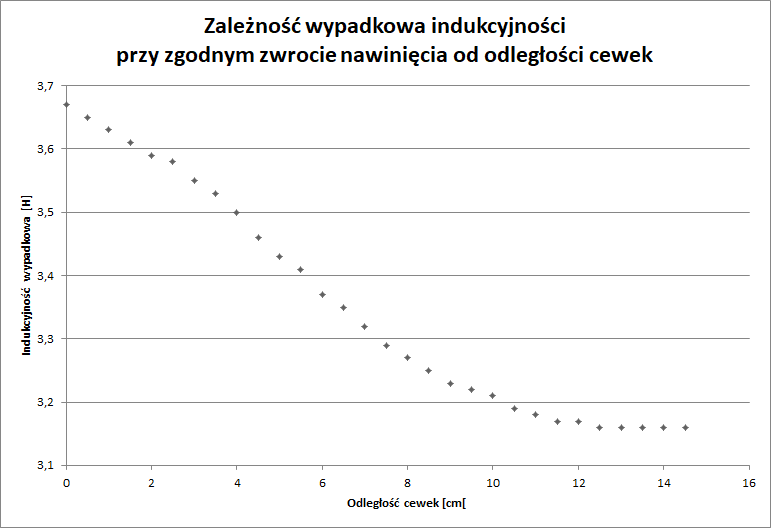
\includegraphics[scale=0.6]{W1}}
	\end{figure}
		\begin{figure}[H]
		\centering{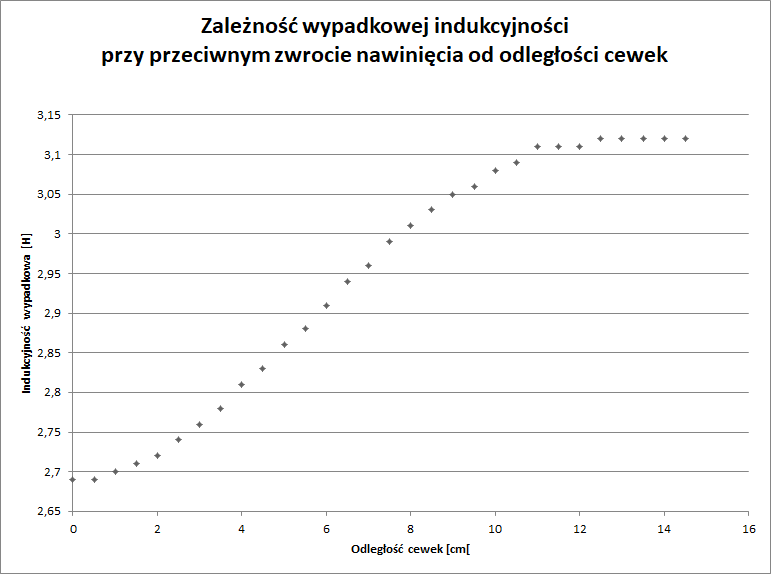
\includegraphics[scale=0.6]{W2}}
	\end{figure}
	\begin{figure}[H]
	\centering{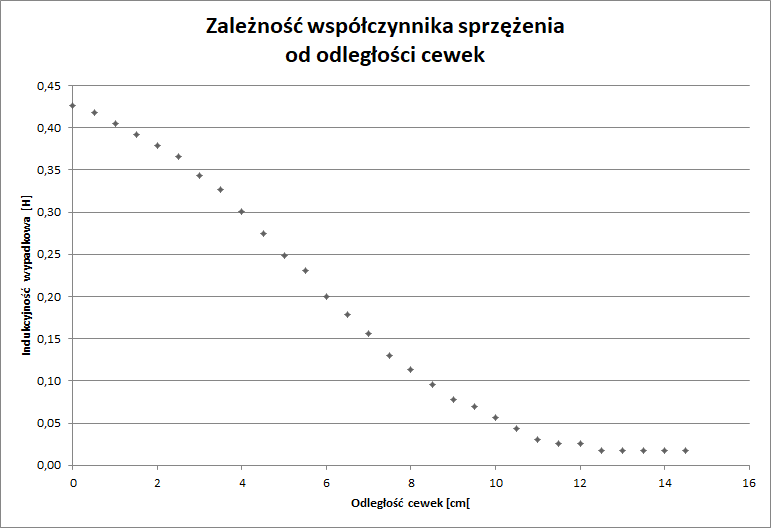
\includegraphics[scale=0.6]{W3}}
	\end{figure}
 \newpage

	\section{Wnioski}

Przy zgodnym zwrocie nawinięcia możemy zauważyć, że wraz ze wzrostem odległości cewki zmniejsza się indukcyjność wypadkowa układu. Natomiast, gdy zwrot nawinięcia jest przeciwny, wraz ze wzrostem odległości cewki zwiększa się indukcyjność wypadkowa.Wraz ze wzrostem odległości cewki zwiększa się współczynnik sprzężenia.\\
Wyniki podane w tabeli mogą różnić się od rzeczywistych ze względu na niepewność miernika cyfrowego. Odczytanie wartości było subiektywne, ponieważ wskaźnik wahał się między wartościami, co wiązało się z koniecznością wyboru odczytanej wartości. Dodatkowo błędy mogły wynikać z konieczności oszacowania odległości cewki, ponieważ wskaźnik nie znajdował się bezpośrednio na miarce, lecz ponad nią.
\end{document}

\end{}